\documentclass[10pt,a4paper]{report}
\usepackage[utf8]{inputenc}
\usepackage{amsmath}
\usepackage{amsfonts}
\usepackage{amssymb}
\usepackage{graphicx}

\begin{document}

\title{English/Spanish Translation \\ with Language Identification - \\ Project Milestone}
\author{Alex Shah}
\date{11/12/17}

\maketitle

\section{Abstract}

  This project's goal is to combine different architectures of neural networks to form a functional English/Spanish translator with the ability to detect the input language and translate to the corresponding opposite language. The resulting product combines a network to classify the input language with a sequence to sequence based recurrent neural networks for creating contextually aware translations.

\section{Introduction}

  Software translation is a massively useful tool to bridge the gap between cultures. Providing a software implementation for translation does not require the entire computation to occur on the device, but rather through training ahead of time. In this way, your cell phone does not need a desktop PC's compute power to leverage neural networks and the advances such technologies have made in machine translation. However, training the network, and the preparation for making a translator, does require a large amount of compute power and time.

  In order to minimize the amount of time required, we can make training more efficient in software translation by training both translation directions simultaneously. By using encoder/decoder as a basis for our model, there is an interim step (or steps) by which languages and context are broken down into mathematical representations that the network is able to use to translate any language to any other. A neural network does not specifically need to train translation from language A to language B and vice versa, but can learn language A to any language based on language A's learned features. 

	By utilizing language agnostic training, we can improve the speed at which we train. Because it's necessary for the model to learn abstracted features of a language, we can train any language in the same time, without needing to retrain or cross train various languages when a need language is added.

\clearpage

\section{Background}

\subsection{Language Classification}

  Classifying a given input is handled by a Convolutional Neural Network (CNN). It is crucial to quickly determine the input language as identifying the language is an intermediary step before translation. However, incorrectly determining the input language will create incorrect translations. Therefore it is important that the classification network is able to quickly but accurately detect the input language.

\subsection{Contextually Aware Translation}

  Strides have been made using deep learning and deep network models for Machine Translation (MT) accuracy, making MT ever more accurate in contextually aware translation. Sequence to Sequence networks (Seq2Seq) are built like an encoder/decoder. The encoded input text is examined to determine the decoded output in the target language. An attention mechanism is used to share information from previous input steps to help better inform output decoding. This is more efficient than bidirectionally sharing input and output values, but is also more accurate than less computationally intensive methods such as reversing input strings. Specifically, attention shares memory between the encoder steps and decoder to produce more contextually aware output.

  Neural Machine Translation (NMT) is a specifically derivated set of Seq2Seq and RNN based models focusing on accuracy and efficiency of training translation models. The encoder mechanisms in NMT models are used to build a thought vector from a given input. This contextual capturing vector of sentence meaning is then decoded into the target language translation. The context captured in this thought vector, in addition to the attention mechanism determining how much is enough or too much context, thus enables the translation to capture and translate advanced syntactical structures such as gender agreement and other "long range dependencies"

\clearpage

\begin{figure}
  \begin{center}
    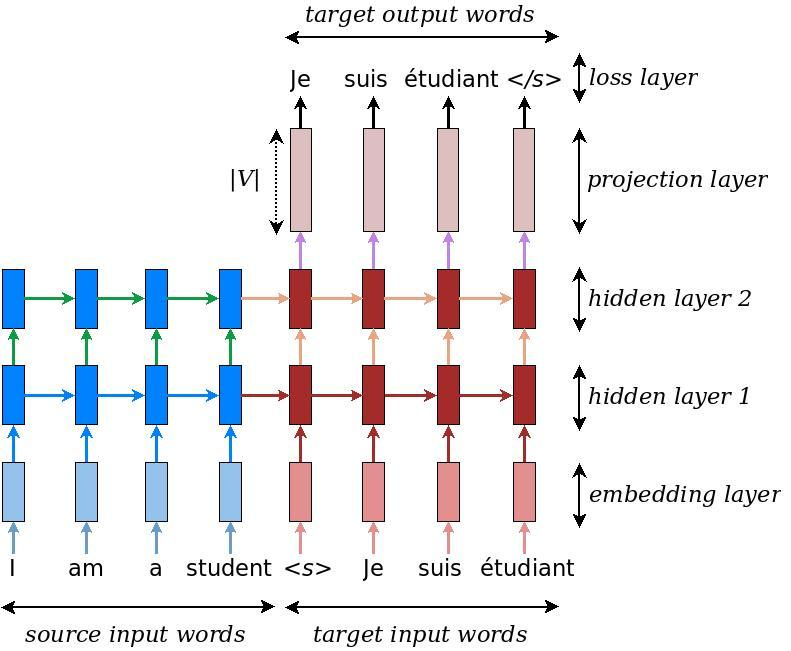
\includegraphics[width=0.8\textwidth]{seq2seq.jpg}
    \caption{Sequence to Sequence Model (Luong, 2017)}
  \end{center}
\end{figure}

\begin{figure}
  \begin{center}
    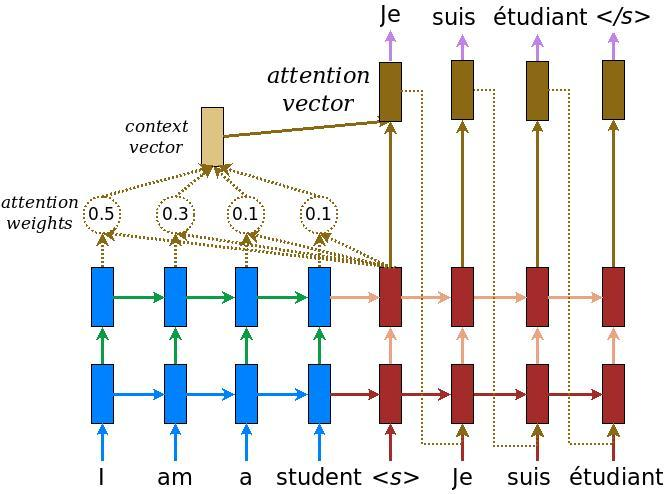
\includegraphics[width=0.8\textwidth] {attention_mechanism.jpg}
    \caption{Sequence to Sequence Model with Attention Mechanism (Luong, 2017)}
  \end{center}
\end{figure}

\clearpage

\section{Methodology}

  In this project there are two networks. A Convolutional Neural Network is used as a language classifier, to detect whether a given input is English or Spanish. Next, a Sequence to Sequence network, specifically using Google's Neural Machine Translation framework translates the given input to the opposite language. For example a given input is identified as English and translated to Spanish. And vice versa. The structure of the program is divided into the two main components. Classify will determine the input language, Translate will translate the input. The main program will use these two functions. Training will be done separately from the application's client facing usage. In this case, the end product will remain a command line interface but can be implemented in an API or web interface easily.

\section{Experiments}

  Datasets in Spanish were difficult to find, but there are many datasets in other languages. In order to train translation, the model needs to study the target language and human corrected translations. In order to translate from one language to another, it is not necesary to train the model withthe input language and human corrected translations of the target language, but rather any human corrected language. In this way a trained model can train on multiple languages without need for datasets to overlap languages, or even add a new language at a later date.

  The data used in this project comes from hand translated European Parliament records dating from 1996 to 2011. The dataset contains nearly 2 million sentences hand translated between English and Spanish.

  The classifier will be trained on the same dataset which the Spanish and English corpuses reach almost 54 million words each.

\clearpage

\section{References}

\subsection{Further Reading}

https://github.com/tensorflow/nmt

https://github.com/google/seq2seq

http://www.nltk.org/

\subsection{Articles}

https://nlp.stanford.edu/projects/nmt/

https://research.googleblog.com/2017/07/building-your-own-neural-machine.html

https://sites.google.com/site/acl16nmt/

https://github.com/lmthang/thesis

https://google.github.io/seq2seq/data/

\subsection{Papers}

https://arxiv.org/pdf/1611.04558v1.pdf

https://papers.nips.cc/paper/5346-sequence-to-sequence-learning-with-neural-networks.pdf

http://aclweb.org/anthology/D/D14/D14-1179.pdf

https://arxiv.org/pdf/1409.0473.pdf

https://arxiv.org/pdf/1508.04025.pdf

https://arxiv.org/abs/1609.08144

https://arxiv.org/abs/1703.01619

\subsection{Data}

http://www.statmt.org/europarl/

https://conferences.unite.un.org/UNCorpus

http://www.statmt.org/wmt17/translation-task.html

\end{document}
